\documentclass[a4paper,14pt]{article}

% Поддержка русского языка
\usepackage[T1, T2A]{fontenc}    % Кодировка
\usepackage[utf8]{inputenc}  % Кодировка исходного текста
\usepackage[english, russian]{babel}  % Локализация и переносы
\usepackage{titlesec, titletoc} % Для настройки стилей заголовков и содержания
\usepackage{booktabs} % Для использования \toprule, \midrule и \bottomrule
\usepackage{array}  % Для лучшего контроля столбцов
\usepackage{cmap}    % Поиск и копирование в PDF
\usepackage{geometry}    % Поля
    \geometry{left=30mm, right=15mm, top=20mm, bottom=20mm}
\usepackage{hhline} % Для двойных линий и более точного контроля границ
\usepackage{caption} % Для настройки подписей
\usepackage{verbatim}
\usepackage{xcolor} % Пакет для цвета
\usepackage{listings} % Пакет для вставки кода
\usepackage{indentfirst}
\usepackage{graphicx}

\usepackage{tikz}

\usetikzlibrary{shapes.geometric, arrows}

\tikzstyle{startstop} = [rectangle, rounded corners, minimum width=3.5cm, minimum height=1cm, text centered, draw=black, fill=red!30]
\tikzstyle{process} = [rectangle, minimum width=3.5cm, minimum height=1cm, text centered, draw=black, fill=blue!20]
\tikzstyle{decision} = [diamond, minimum width=3.5cm, minimum height=1cm, text centered, draw=black, fill=green!30]
\tikzstyle{arrow} = [thick,->,>=stealth]

% \usepackage{times}

% Установка стандартного отступа (2em)
\setlength{\parindent}{2em}

% Установка отступа после заголовков
\usepackage{titlesec}
\titlespacing*{\section}{0pt}{2\baselineskip}{\baselineskip}
\titlespacing*{\subsection}{0pt}{2\baselineskip}{\baselineskip}
\titlespacing*{\subsubsection}{0pt}{2\baselineskip}{\baselineskip}

% Определение цветов
% \definecolor{operatorcolor}{HTML}{ED028C}
% \definecolor{stringcolor}{HTML}{9400D1}
% \definecolor{commentcolor}{HTML}{005000}
% \definecolor{backgroundcolor}{HTML}{fafafa}
\definecolor{backgroundcolor}{HTML}{fafafa} % Темный фон
\definecolor{keywordcolor}{rgb}{0.86, 0.58, 0.35} % Ключевые слова (оранжевый)
\definecolor{stringcolor}{rgb}{0.72, 0.92, 0.53} % Строки (зеленый)
\definecolor{commentcolor}{HTML}{005000} % Комментарии (серый)
\definecolor{numbercolor}{rgb}{0.75, 0.75, 0.75} % Номера строк (светло-серый)
\definecolor{identifiercolor}{rgb}{0.60, 0.60, 1.00} % Идентификаторы (светло-синий)
\definecolor{keywordtypcolor}{rgb}{0.57, 0.81, 1.00} % Типы данных (голубой)

% Настройка подсветки синтаксиса
\lstset{
    language=[x86masm]Assembler,
   basicstyle=\ttfamily\fontsize{10}{12}\selectfont, % Моноширный основной стиль текста
   backgroundcolor=\color{backgroundcolor}, % Цвет фона
   % commentstyle=\color{commentcolor}\itshape, % Стиль комментариев
    numbers=left,
    numberstyle=\tiny,
    stepnumber=1,
    showstringspaces=false,
    tabsize=2,
    breaklines=true, % Автоматический перенос строк
    postbreak=\mbox{\textcolor{red}{$\hookrightarrow$}\space},
    frame=none, % Убрать рамку вокруг кода
    captionpos=b, % Заголовок (caption) снизу и центрирован
    literate=% Поддержка кириллицы в комментариях (маленькие и большие буквы)
    {а}{{\selectfont\char224}}1
    {б}{{\selectfont\char225}}1
    {в}{{\selectfont\char226}}1
    {г}{{\selectfont\char227}}1
    {д}{{\selectfont\char228}}1
    {е}{{\selectfont\char229}}1
    {ё}{{\"e}}1
    {ж}{{\selectfont\char230}}1
    {з}{{\selectfont\char231}}1
    {и}{{\selectfont\char232}}1
    {й}{{\selectfont\char233}}1
    {к}{{\selectfont\char234}}1
    {л}{{\selectfont\char235}}1
    {м}{{\selectfont\char236}}1
    {н}{{\selectfont\char237}}1
    {о}{{\selectfont\char238}}1
    {п}{{\selectfont\char239}}1
    {р}{{\selectfont\char240}}1
    {с}{{\selectfont\char241}}1
    {т}{{\selectfont\char242}}1
    {у}{{\selectfont\char243}}1
    {ф}{{\selectfont\char244}}1
    {х}{{\selectfont\char245}}1
    {ц}{{\selectfont\char246}}1
    {ч}{{\selectfont\char247}}1
    {ш}{{\selectfont\char248}}1
    {щ}{{\selectfont\char249}}1
    {ъ}{{\selectfont\char250}}1
    {ы}{{\selectfont\char251}}1
    {ь}{{\selectfont\char252}}1
    {э}{{\selectfont\char253}}1
    {ю}{{\selectfont\char254}}1
    {я}{{\selectfont\char255}}1
    {А}{{\selectfont\char192}}1
    {Б}{{\selectfont\char193}}1
    {В}{{\selectfont\char194}}1
    {Г}{{\selectfont\char195}}1
    {Д}{{\selectfont\char196}}1
    {Е}{{\selectfont\char197}}1
    {Ё}{{\"E}}1
    {Ж}{{\selectfont\char198}}1
    {З}{{\selectfont\char199}}1
    {И}{{\selectfont\char200}}1
    {Й}{{\selectfont\char201}}1
    {К}{{\selectfont\char202}}1
    {Л}{{\selectfont\char203}}1
    {М}{{\selectfont\char204}}1
    {Н}{{\selectfont\char205}}1
    {О}{{\selectfont\char206}}1
    {П}{{\selectfont\char207}}1
    {Р}{{\selectfont\char208}}1
    {С}{{\selectfont\char209}}1
    {Т}{{\selectfont\char210}}1
    {У}{{\selectfont\char211}}1
    {Ф}{{\selectfont\char212}}1
    {Х}{{\selectfont\char213}}1
    {Ц}{{\selectfont\char214}}1
    {Ч}{{\selectfont\char215}}1
    {Ш}{{\selectfont\char216}}1
    {Щ}{{\selectfont\char217}}1
    {Ъ}{{\selectfont\char218}}1
    {Ы}{{\selectfont\char219}}1
    {Ь}{{\selectfont\char220}}1
    {Э}{{\selectfont\char221}}1
    {Ю}{{\selectfont\char222}}1
    {Я}{{\selectfont\char223}}1
}

\captionsetup[table]{justification=raggedright, singlelinecheck=false} % Выравнивание подписи по левому краю

% Установка стиля заголовков разделов: центрирование без номера
\titleformat{\section}[block]{\Large\bfseries\centering}{}{0pt}{}

\title{3.1 Титульный лист}

\begin{document}

\thispagestyle{empty}    % Отключаем колонтитулы

\begin{center}
    Санкт-Петербургский политехнический университет Петра Великого\\
    Институт компьютерных наук и технологий\\
    \bfseries{Высшая школа программной инженерии}
\end{center}

\vspace{20ex} % Задаем размер вертикального промежутка в явном виде

\begin{center}
    \begin{huge} {\bfseries{\scshape курсовая работа}} \end{huge}

    \vspace{3ex}
    \textbf{Программирование на языке Ассемблера}\\
    по дисциплине: «Архитектура компьютера»
\end{center}

\vspace{30ex}

\noindent Выполнила\\
студентка гр. в5130904/30022\hfill \begin{minipage}{0.6\textwidth} \hfill Г.М.Феллер\end{minipage}

\vspace{3ex}

\noindent Руководитель\\
проф, д.т.н.\hfill \begin{minipage} {0.6\textwidth}\hfill С.А.Молодяков\end{minipage}

\vspace{3ex}

\hfill \begin{minipage}{0.6\textwidth} \hfill «\underline{\hspace{1cm}}»\underline{\hspace{3cm}} 2024 г.\end{minipage}

\vfill

\begin{center}
    Санкт-Петербург\\ 
    2024
\end{center}

\newpage % Начинаем новую страницу\

% Отключение нумерации разделов в заголовках разделов и подразделов
\titleformat{\section}[block]{\Large\bfseries\centering}{}{0pt}{}

% Настройка заголовков подразделов с использованием символа "§" и собственной нумерации
\renewcommand{\thesubsection}{\S\arabic{subsection}}
\titleformat{\subsection}[block]{\large\bfseries}{\thesubsection}{1em}{}
% Установка автоматического сброса счетчика подразделов при начале нового раздела

% Определение стиля оглавления
\titlecontents{section}[0pt] % Left indent
{\vspace{0.5ex}\hspace{1em}} % Above code and left spacing
{} % Numbered entry format (empty to remove numbers)
{} % Numberless entry format
{\titlerule*[1pc]{.}\contentspage} % Filler-page format

% Настройка стиля заголовка Содержания с выравниванием по левому краю
\renewcommand{\contentsname}{\leftline{\fontsize{24.5pt}{30pt}\selectfont Содержание}}

\tableofcontents

\newpage

\section{Введение}

Язык программирования ассемблер относится к категории низкоуровневых и предназначен для работы с машинным кодом. Его структура и функции определяются архитектурой процессора и особенностями вычислительной системы. Ассемблер дает возможность взаимодействовать с аппаратным обеспечением компьютера на прямом уровне. Программы, написанные на ассемблере, состоят из инструкций, которые в процессе трансляции преобразуются в машинные коды. \newline

\paragraph{Задание \newline}
Дан список из 20 слов по 10 символов в каждом. Напечатать его в
обратном алфавитном порядке, предварительно удалив из него
повторяющиеся слова. При сортировке игнорировать высоту букв
(Например, A = a).

\newpage

\section{Блок-схема}
\paragraph{Структура програмы \newline\newline}
\begin{tikzpicture}[node distance=2cm]

    % Nodes
    \node (start) [startstop] {Начало программы};
    \node (init) [process, below of=start] {Инициализация сегментов};
    \node (printarray) [process, below of=init] {Вывод массива строк (PrintStrings)};
    \node (sort) [process, below of=printarray] {Сортировка строк (SortStrings)};
    \node (printsorted) [process, below of=sort] {Вывод отсортированного массива};
    \node (end) [startstop, below of=printsorted] {Завершение программы};

    % Arrows
    \draw [arrow] (start) -- (init);
    \draw [arrow] (init) -- (printarray);
    \draw [arrow] (printarray) -- (sort);
    \draw [arrow] (sort) -- (printsorted);
    \draw [arrow] (printsorted) -- (end);

\end{tikzpicture}
\newpage
\paragraph{Алгоритм сортировки \newline\newline}
\begin{tikzpicture}[node distance=2.5cm]

    % Nodes
    \node (start) [startstop] {Начало сортировки};
    \node (outerloop) [process, below of=start] {Инициализация внешнего цикла (SI)};
    \node (innerloop) [process, below of=outerloop] {Инициализация внутреннего цикла (DI)};
    \node (compare) [process, below of=innerloop] {Сравнение строк (Compare2Strings)};
    \node (decision) [decision, below of=compare, yshift=-1cm] {Порядок строк нарушен?};
    \node (swap) [process, right of=decision, xshift=5cm] {Перестановка строк};
    \node (checkinner) [decision, below of=decision, yshift=-2cm] {DI достиг конца?};
    \node (checkouter) [decision, below of=checkinner, yshift=-2cm] {SI достиг конца?};
    \node (end) [startstop, below of=checkouter, yshift=-1cm] {Конец сортировки};
    
    % Arrows
    \draw [arrow] (start) -- (outerloop);
    \draw [arrow] (outerloop) -- (innerloop);
    \draw [arrow] (innerloop) -- (compare);
    \draw [arrow] (compare) -- (decision);
    \draw [arrow] (decision.east) -- (swap.west) node[midway, above] {Да};
    \draw [arrow] (swap.south) |- (checkinner);
    \draw [arrow] (decision.south) -- (checkinner) node[midway, right] {Нет};
    \draw [arrow] (checkinner.south) -- (checkouter) node[midway, right] {Да};
    \draw [arrow] (checkinner.west) -- ++(-3cm,0) |- (innerloop) node[midway, above] {Нет};
    \draw [arrow] (checkouter.south) -- (end) node[midway, right] {Да};
    \draw [arrow] (checkouter.west) -- ++(-2cm,0) |- (outerloop) node[midway, above] {Нет};
    
\end{tikzpicture}


\newpage

\section{Список использованных прерываний BIOS}

\textbf{INT 21h} – Main DOS API

\begin{table}[h]
    \centering
    \begin{tabular}{|m{2cm}|m{10cm}|} 
        \hline
        \textbf{AH} & \textbf{Description} \\ % Заголовки столбцов
        \hline
        09h  & Display string   \\ 
        \hline
        20h & Terminate the current program \\ 
        \hline
        4C00h & Terminate with return code 0 \\ 
        \hline
    \end{tabular}
    \label{tab:dos} % Ссылка на таблицу
\end{table}

\newpage

\section{Листинг кода}

\begin{lstlisting}
Name words
; Сегмент данных: строки, указатели и вспомогательные данные
data segment
db "Scepticism",9,"$"
db "acceptance",9,"$"
db "yellowwood",9,"$"
db "Conversion",9,"$"
db "management",9,"$"
db "Corruption",9,"$"
db "depression",9,"$"
db "collection",9,"$"
db "investment",9,"$"
db "assembling",9,"$"
db "Management",9,"$"
db "conversion",9,"$"
db "obligation",9,"$"
db "prospectus",9,"$"
db "Collection",9,"$"
db "securities",9,"$"
db "Investment",9,"$"
db "typewriter",9,"$"
db "Validation",9,"$"
db "xenogenies",9,"$"

; Смещения начала каждой строки 
stringarr dw 0,12,24,36,48,60,72,84,96,108,120,132,144,156,168,180,192,204,216,228
; Количество строк в массиве
stringnum dw 20
; Вывод заголовков
array db 'Array:',13,10,'$'
result db 13,10,'Result:',13,10,'$'
data ends
    
; Сегмент стека: используется для временного хранения данных
stacks segment word stack 'stack'
; Выделение 200 слов для стека
dw 200 dup(?) 
; Указатель на вершину стека
StackTop:
stacks ends 

; Сегмент кода программы
code segment
; Указываем, что CS, DS, ES, SS указывают на свои сегменты
assume CS: code, DS: data, ES: data, SS: stacks

; Процедура PrintStrings: выводит на экран строки из массива
PrintStrings proc
    push bp         ; Сохраняем базовый указатель
    mov bp,sp       ; Устанавливаем стек-кадр
    push si         ; Сохраняем регистр SI
    push di         ; Сохраняем регистр DI
    push dx         ; Сохраняем регистр DX
    push cx         ; Сохраняем регистр DI

    mov si,[bp+4]   ; Указатель на массив строк (stringarr)
    mov di,[bp+6]   ; Указатель на количество строк (stringnum)
    mov cx,[di]     ; Количество строк

    print:
    mov dx,[si]     ; Адрес текущей строки
    mov ah,09h      ; Функция DOS (09h - вывод строки)
    int 21h         ; Вызов DOS для вывода строки
    add si,2        ; Переход к следующему указателю в stringarr
    loop print      ; Уменьшаем CX и повторяем цикл, если CX > 0

    pop cx          ; Восстанавливаем регистр CX
    pop dx          ; Восстанавливаем регистр DX
    pop di          ; Восстанавливаем регистр DI
    pop si          ; Восстанавливаем регистр SI
    pop bp          ; Восстанавливаем базовый указатель
    ret 4           ; Выход из процедуры
PrintStrings endp

; Процедура Compare2Strings: сравнивает две строки
Compare2Strings proc
    push bp         ; Сохраняем базовый указатель
    mov bp,sp       ; Устанавливаем стек-кадр
    push si         ; Сохраняем регистр SI
    push di         ; Сохраняем регистр DI
    push cx         ; Сохраняем регистр CX
    push dx         ; Сохраняем регистр DX

    mov si,[bp+4]   ; SI = указатель на первую строку
    mov di,[bp+6]   ; DI = указатель на вторую строку
    mov cx,10       ; CX = количество символов сравнения

    startcom:
    lodsb           ; Загружаем текущий символ первой строки в AL
    cmp al,'a'      ; Проверяем, меньше ли символ 'a'
    jb readsymstr2  ; Если меньше, пропускаем преобразование
    cmp al,'z'      ; Проверяем, больше ли символ 'z'
    ja readsymstr2  ; Если больше, пропускаем преобразование
    sub al,20h      ; Преобразуем символ в верхний регистр

    readsymstr2:
    mov ah,[di]     ; Загружаем символ второй строки в AH
    inc di          ; Увеличиваем DI для перехода к следующему символу
    cmp ah,'a'      ; Проверяем, меньше ли символ 'a'
    jb comparesym   ; Если меньше, пропускаем преобразование
    cmp ah,'z'      ; Проверяем, больше ли символ 'z'
    ja comparesym   ; Если больше, пропускаем преобразование
    sub ah,20h      ; Преобразуем символ в верхний регистр

    comparesym:
    cmp al,ah       ; Сравниваем символы
    jz nextsym      ; Если равны, переходим к следующему
    ja above        ; Если первый символ больше, переходим к "above"
    mov al,1        ; Устанавливаем результат = 1 (меньше)
    jmp exit

    above:
    mov al,2        ; Устанавливаем результат = 2 (больше)	
    jmp exit

    nextsym:
    loop startcom   ; Повторяем цикл для всех символов
    mov al,0        ; Если строки равны, результат = 0

    exit:
    pop dx          ; Восстанавливаем регистр DX
    pop cx          ; Восстанавливаем регистр CX
    pop di          ; Восстанавливаем регистр DI
    pop si          ; Восстанавливаем регистр SI
    pop bp          ; Восстанавливаем базовый указатель
    ret 4           ; Выход из процедуры
Compare2Strings endp
    
; Процедура RemoveDuplicate: удаляет дублирующую строку
RemoveDuplicate proc
    push bp         ; Сохраняем базовый указатель
    mov bp,sp       ; Устанавливаем стек-кадр
    push si         ; Сохраняем регистр SI
    push di         ; Сохраняем регистр DI

    mov di,[bp+8]   ; DI = указатель на stringnum
    mov ax,[di]     ; AX = количество строк
    dec ax          ; Уменьшаем количество строк
    mov [di],ax     ; Обновляем stringnum

    mov si,[bp+6]   ; SI = конец массива строк
    mov di,[bp+4]   ; DI = текущая строка

    cmp si,di       ; Проверка, достигнут ли конец массива       
    jz exitdup      ; Если достигнут, выходим

    moving:           
    mov ax,[di+2]   ; Копируем следующую строку в текущую
    mov [di],ax
    add di,2        ; Переходим к следующей строке
    cmp di,si       ; Проверяем, достигнут ли конец массива
    jb moving       ; Если нет, продолжаем

    exitdup:
    pop di          ; Восстанавливаем регистр DI
    pop si          ; Восстанавливаем регистр SI
    pop bp          ; Восстанавливаем базовый указатель
    ret 6           ; Выход из процедуры
RemoveDuplicate endp
    
; Процедура SortStrings: сортирует строки в массиве stringarr в алфавитном порядке
SortStrings proc
    push bp         ; Сохраняем базовый указатель
    mov bp,sp       ; Устанавливаем стек-кадр
    push si         ; Сохраняем регистр SI
    push di         ; Сохраняем регистр DI
    push cx         ; Сохраняем регистр CX
    push bx         ; Сохраняем регистр BX
    push dx         ; Сохраняем регистр DX

    mov si,[bp+4]   ; SI = указатель на начало массива строк (stringarr)
    mov di,[bp+6]   ; DI = указатель на количество строк (stringnum)
    mov ax,[di]     ; AX = количество строк 
    dec ax          ; AX = количество строк - 1 (для границ сортировки)
    shl ax,1        ; Умножаем AX на 2 (каждый указатель занимает 2 байта)
    mov dx,si       ; DX = начало массива строк
    add dx,ax       ; DX = конец массива строк

    sort:
    mov di,si       ; DI = указатель на текущую строку (начало текущего прохода)
    add di,2        ; DI = указатель на следующую строку

    sort2:
    push [di]       ; Сохраняем указатель на строку 2
    push [si]       ; Сохраняем указатель на строку 1

    ; Вызов процедуры сравнения строк
    call Compare2Strings

    cmp al,0        ; Проверяем результат сравнения
    jne check1      ; Если строки не равны, переходим к следующей проверке

    ; Удаление дублирующейся строки
    push [bp+6]     ; Передаем указатель на stringnum
    push dx         ; Передаем конец массива строк
    push di         ; Передаем указатель на дублирующуюся строку

    ; Вызов процедуры удаления дублирующейся строки
    call RemoveDuplicate

    sub dx,2        ; Сдвигаем конец массива строк
    cmp di,dx       ; Проверяем, достиг ли DI конца массива
    jbe sort2       ; Если нет, продолжаем сортировку

    jmp exitremove  ; Переходим к завершению процедуры

    check1:
    cmp al,1        ; Проверяем, первая строка меньше второй?	
    jne next        ; Если нет, переходим к следующей строке

    ; Обмен строк местами
    mov bx,[di]     ; BX = указатель на строку 2
    mov cx,[si]     ; CX = указатель на строку 1
    mov [di],cx     ; Меняем местами указатели строк
    mov [si],bx     ; Завершаем обмен

    next:
    add di,2        ; DI = следующая строка
    cmp di,dx       ; Проверка, достиг ли DI конца массива
    jbe sort2       ; Если нет, продолжаем сортировку текущего прохода

    add si,2        ; SI = следующая строка для нового прохода
    cmp si,dx       ; Проверка, достиг ли SI конца массива
    jb sort         ; Если нет, продолжаем сортировку

    exitremove:
    pop dx          ; Восстанавливаем регистр DX
    pop bx          ; Восстанавливаем регистр BX
    pop cx          ; Восстанавливаем регистр CX
    pop di          ; Восстанавливаем регистр DI
    pop si          ; Восстанавливаем регистр SI
    pop bp          ; Восстанавливаем базовый указатель
    ret 4           ; Выход из процедуры
SortStrings endp

; Начало выполнения программы
start: 
    mov sp,offset StackTop  ; Инициализация указателя стека (SP) на вершину стека

    ; Инициализация сегментов данных
    mov ax,data             
    mov ds,ax		
    mov es,ax		

    ; Вывод заголовка "Array:"
    mov dx,offset array     ; DX = адрес строки
    mov ah,09h              ; Функция DOS (09h - вывод строки)
    int 21h                 ; Вызов DOS для вывода строки

    ; Вывод массива строк перед сортировкой
    lea ax,stringnum        ; AX = адрес количества строк
    push ax                 ; Передаем адрес количесвта строк в стек
    lea ax,stringarr        ; AX = адрес массива строк
    push ax                 ; Передаем адрес массива строк в стек
    call PrintStrings       ; Вызов процедуры PrintStrings

    ; Вывод заголовка "Result:"
    mov dx,offset result    ; DX = адрес строки
    mov ah,09h              ; Функция DOS (09h - вывод строки)
    int 21h                 ; Вызов DOS для вывода строки

    ; Сортировка массива строк
    lea ax,stringnum        ; AX = адрес количества строк
    push ax                 ; Передаем адрес количесвта строк в стек
    lea ax,stringarr        ; AX = адрес массива строк
    push ax                 ; Передаем адрес массива строк в стек
    call SortStrings        ; Вызов процедуры SortStrings

    ; Вывод массива строк после сортировки
    lea ax,stringnum        ; AX = адрес количества строк
    push ax                 ; Передаем адрес количества строк в стек
    lea ax,stringarr        ; AX = адрес массива строк
    push ax                 ; Передаем адрес массива в стек
    call PrintStrings       ; Вызываем процедуру PrintStrings

    ; Завершение программы
    mov ax,4c00h            ; Функция DOS (4Ch - завершение программы)
    int 21h                 ; Вызов DOS для завершения программы

code ends
end start
\end{lstlisting}

\newpage

\section{Пример выполнения программы}

\begin{figure}[h] % Окружение figure для оформления картинки
    \centering % Центровка картинки
    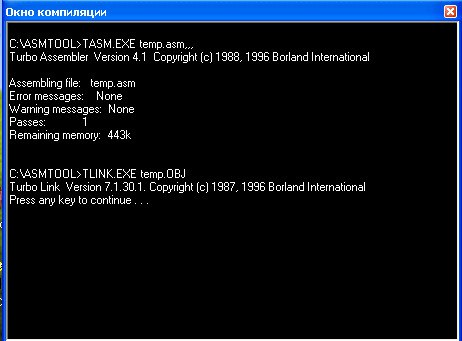
\includegraphics[width=0.7\textwidth]{compiler.jpg} % Вставка картинки, ширина 70% текста
    \caption{Окно компиляции программы} % Подпись к картинке
    \label{fig:compiler} % Ссылка для использования в тексте
\end{figure}

\begin{figure}[h] % Окружение figure для оформления картинки
    \centering % Центровка картинки
    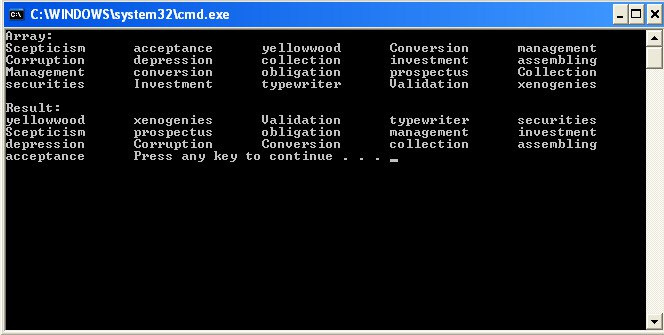
\includegraphics[width=0.7\textwidth]{exe.jpg} % Вставка картинки, ширина 70% текста
    \caption{Окно выполнения программы} % Подпись к картинке
    \label{fig:exe} % Ссылка для использования в тексте
\end{figure}

\end{document}